\section{The plug-in}
Here a step by step explanation will guide the user through the proper usage of the preditcion plug-in.

\subsection{Loading the plug-in}
\begin{enumerate}
	\item The user will have to select the plus icon from the sidebar, from which a drop-down menu containing four options will appear; from this menu the “dashboard” option has to be selected;


\begin{figure}[H]
\centering
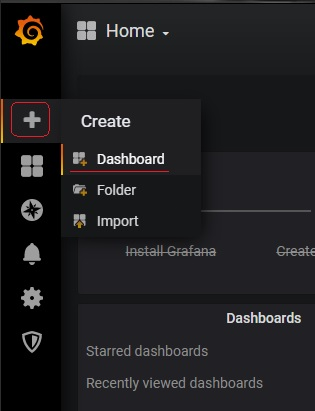
\includegraphics[scale=0.90]{img/plug-in/plus_dash.jpg}
\caption{Training operation with graphic point}
\end{figure}


	\item The user will now have to select the “Chose Visualization” button;


\begin{figure}[H]
\centering
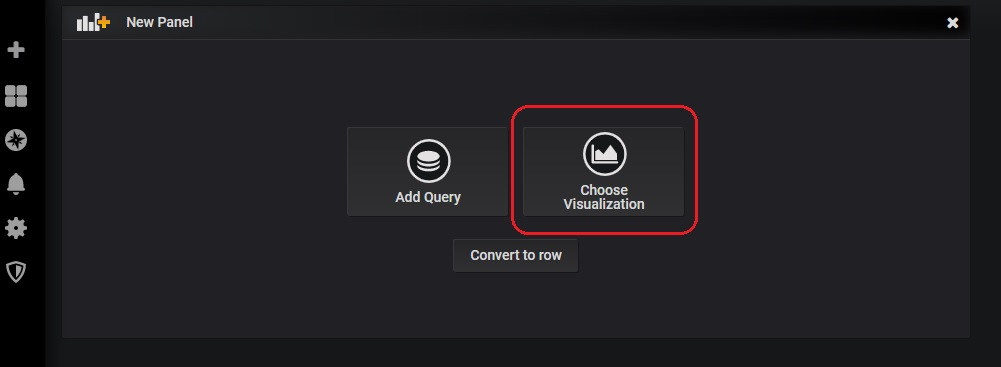
\includegraphics[scale=0.65]{img/plug-in/visual.jpg}
\caption{Chose Visualization button}
\end{figure}


	\item Finally, by pressing on the “Predire in Grafana” button, the user can use the plug-in.
	
\begin{figure}[H]
\centering
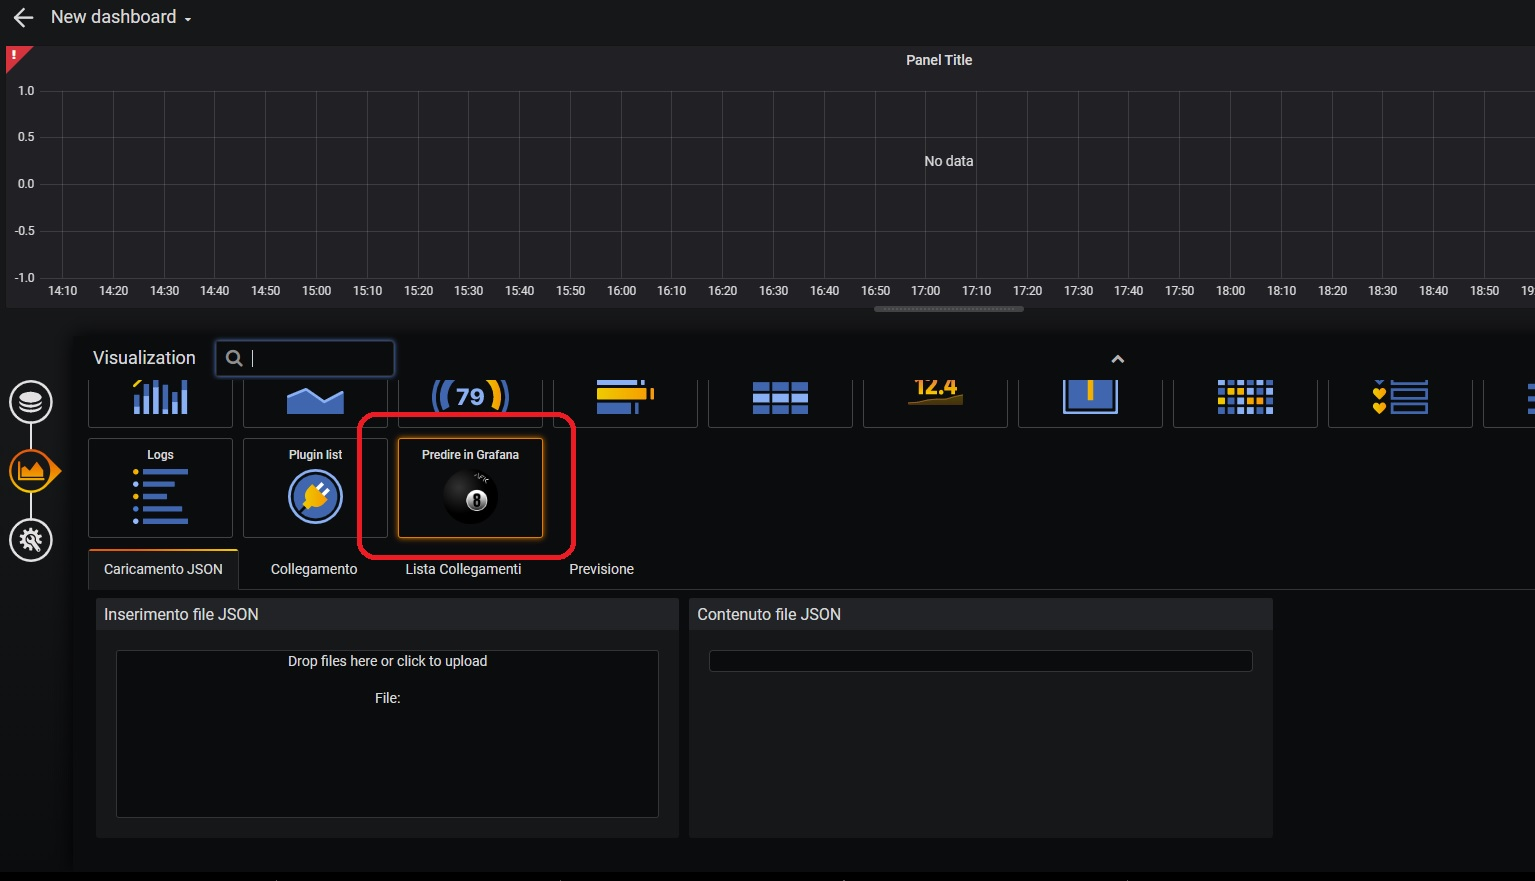
\includegraphics[scale=0.55]{img/plug-in/selection_ball.jpg}
\caption{"Predire in Grafana" Panel}
\end{figure}

\end{enumerate}

	
\subsection{Loading a JSON file}
The user can select the “Inserimento file JSON” button contained in the “Caricamento JSON” section.
This will open a window from which the JSON file can be selected.
Alternatively, the user can drag and drop the JSON file in the "Inserimento file JSON" section.
The content of the JSON file will be displayed in a panel called "Contenuto file JSON" to the right of the previously mentioned section.

\begin{figure}[H]
\centering
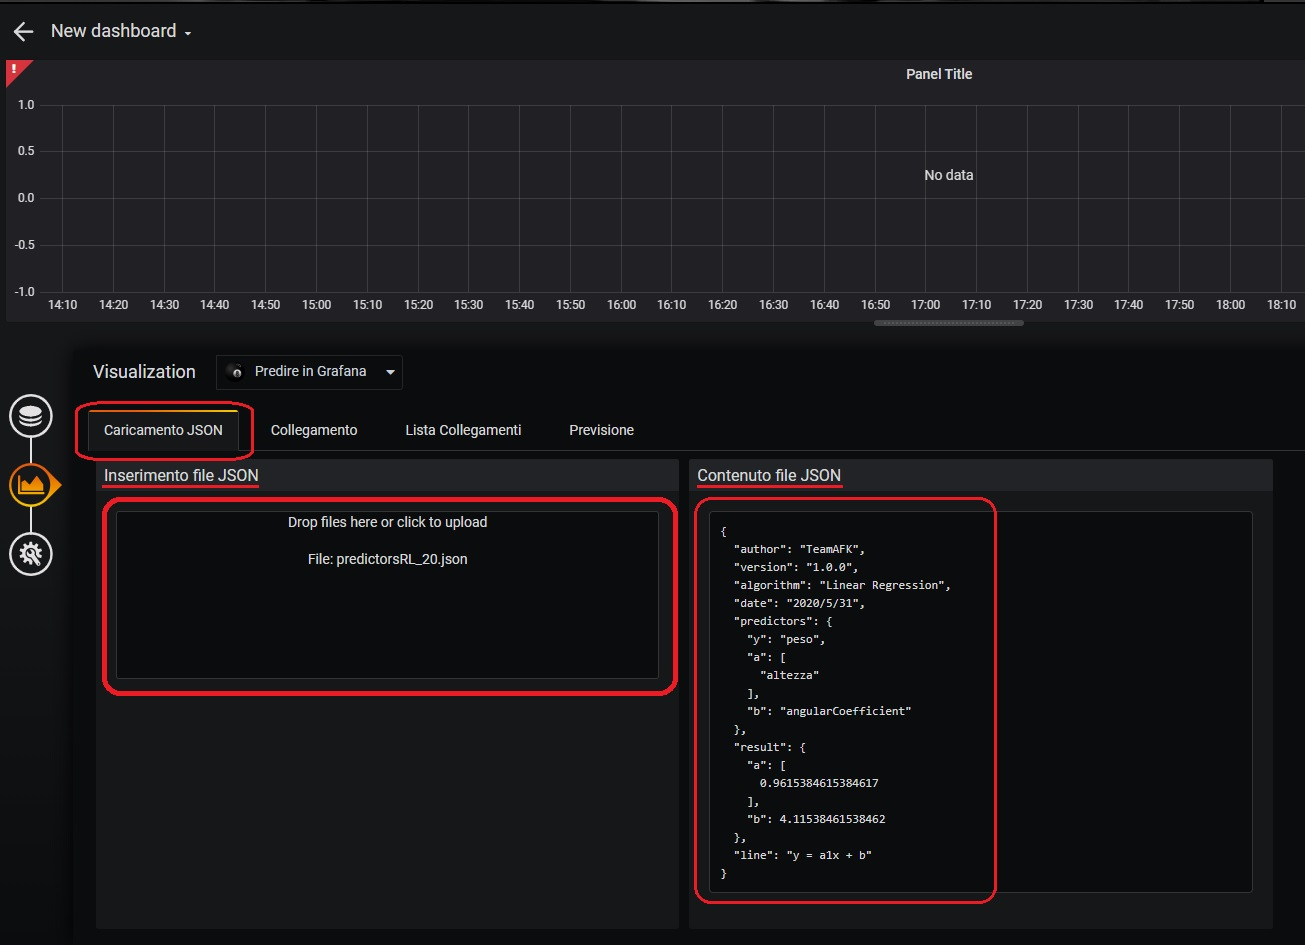
\includegraphics[scale=0.65]{img/plug-in/loading_js.jpg}
\caption{Loading window and displayed loaded JSON}
\end{figure}


\subsection{Connecting the nodes}
The portion of the software dedicated to the connection of the nodes can be accessed by selecting the "Collegamento" tab.
\begin{enumerate}
	\item The user can choose from the “Lista predittori” section which queries are to be associated with which nodes, by selecting a particular query to the right of a predictor: this can be done by opening the drop-down menu tagged with "Seleziona il nodo" and then selecting a query.
	Once all the nodes are connected, the user can select the "Inserisci collegamento" button and confirm the operation;
	
\begin{figure}[H]
\centering
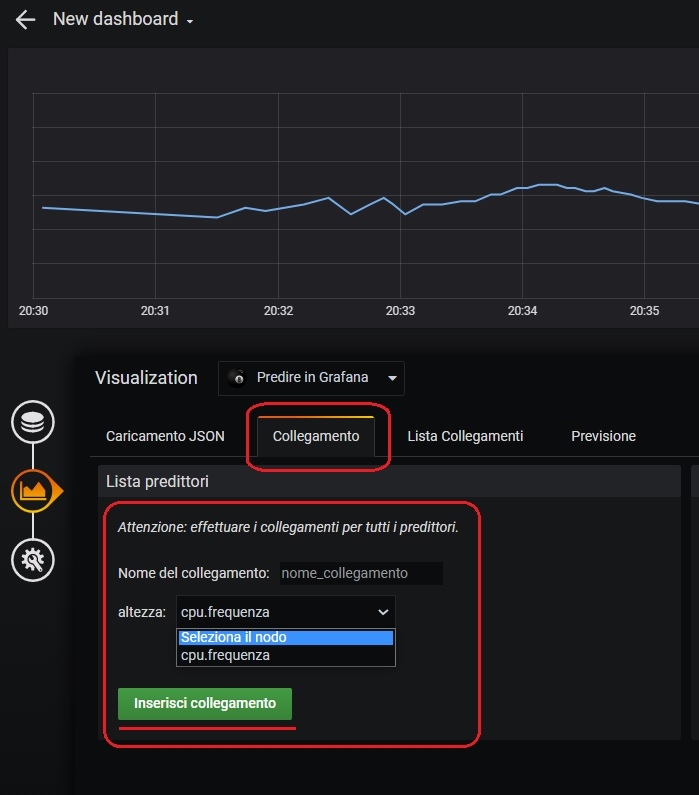
\includegraphics[scale=0.75]{img/plug-in/insert_node.jpg}
\caption{Node coupling (a)}
\end{figure}



\begin{enumerate}
\item Should the user have not filled all the required fields, an error message will be displayed on selection of the "Inserisci collegamento" button;

	
\begin{figure}[H]
\centering
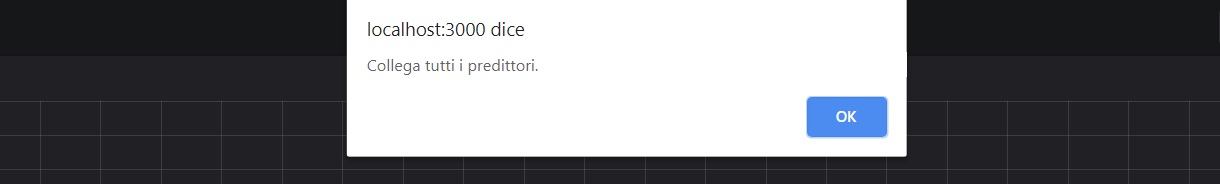
\includegraphics[scale=0.60]{img/plug-in/err_msg.jpg}
\caption{Node coupling error message}
\end{figure}

\item Once all the required fields are correctly chosen, a confirm message will be displayed. 

\begin{figure}[H]
\centering
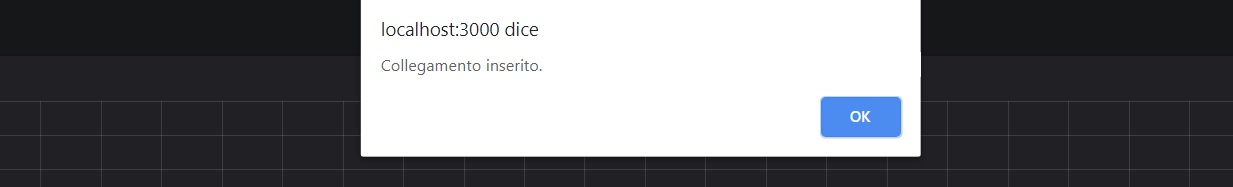
\includegraphics[scale=0.60]{img/plug-in/ok_msg.jpg}
\caption{Node coupling confirm message}
\end{figure}

\end{enumerate} 

	
	\item Maximum and minimum thresholds can be set in the “Impostazione soglie” section, by inserting numbers in the dedicated boxes and then selecting the "Conferma Collegamento" button.


\begin{figure}[H]
\centering
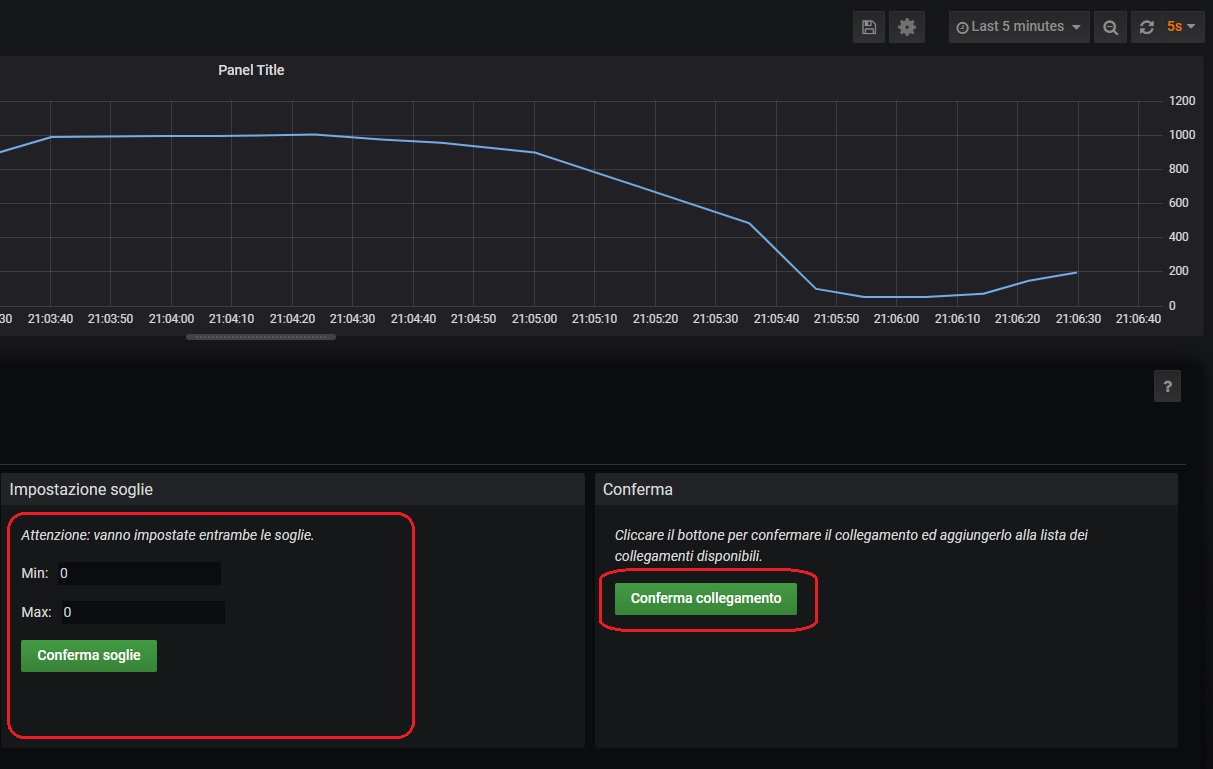
\includegraphics[scale=0.65]{img/plug-in/confirm.jpg}
\caption{Node coupling (b)}
\end{figure}

\end{enumerate}



\subsection{Modifying the connections}
In this section the user can view all the predictor-data stream connections that have been made. This section can be accessed by selecting the "Lista Collegamenti" tab.
The user can also modify the connection, by pressing on the "Modifica Collegamento" button, or delete it, by selecting the "Elimina Collegamento" button.

\begin{figure}[H]
\centering
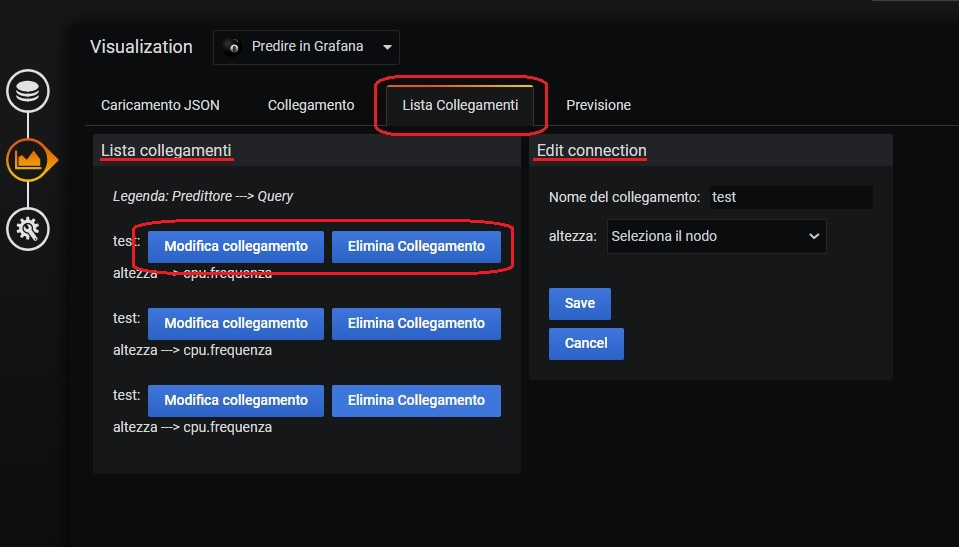
\includegraphics[scale=0.75]{img/plug-in/collegamento_node.jpg}
\caption{Node linking}
\end{figure}


\subsection{Prediction operations}
In this last section the user will be able to launch the prediction algorithms of the plug-in. This section is accessed by selecting the "Previsione" tab. Here the user will be able to select, in the top rigth corner, a temporal policy by choosing starting and ending dates and choosing how often to sample the data. The user  also has access to two buttons, one called "Avvia monitoraggio", which starts the prediction operations, and a second one named "Salva previsione", which saves the data collected up to the point it is pressed.\\

\begin{figure}[H]
\centering
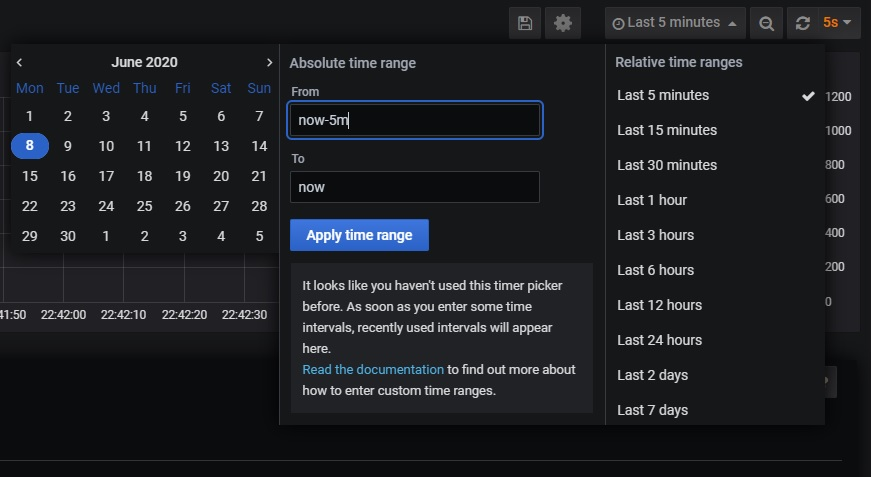
\includegraphics[scale=0.95]{img/plug-in/time_selector.jpg}
\caption{Time picker}
\end{figure}

When the prediction has been started, the "Avvia monitoraggio" button becomes "Interrompi monitoraggio", which, if pressed, will stop the monitoring.

\begin{figure}[H]
\centering
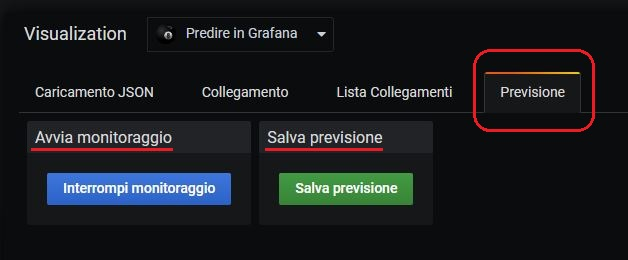
\includegraphics[scale=0.95]{img/plug-in/save_previsione.jpg}
\caption{Begin\textbackslash end data monitoring and Prdicton save}

\end{figure} 
 

